
\documentclass[11pt]{article}

\usepackage{hyperref}
\usepackage{geometry}
\usepackage{listliketab}
\usepackage{array}
\usepackage{longtable}

\usepackage{natbib}
\usepackage{bibentry}
\usepackage{enumitem}
\usepackage{epigraph}
\usepackage{graphicx}
%\usepackage{/Users/hpm/D_DRIVE/latex/enumitem/enumitem}
\nobibliography*
%\bibliographystyle{apa}

% Palatino font
%\usepackage[T1]{fontenc}
%\usepackage[sc,osf]{mathpazo}

\def\name{Marshall Retrospectus / Prospectus}

\reversemarginpar

\geometry{
  body={6.5in, 9in},
  left=0.75in,
  top=0.75in
}

% Customize page headers
\pagestyle{myheadings}
\markright{\name}
%\thispagestyle{empty}

% Custom section fonts
\usepackage{sectsty}
\sectionfont{\rmfamily\mdseries\Large}
\subsectionfont{\rmfamily\mdseries\itshape\large}

% Other possible font commands include:
% \ttfamily for teletype,
% \sffamily for sans serif,
% \bfseries for bold,
% \scshape for small caps,
% \normalsize, \large, \Large, \LARGE sizes.

% Don't indent paragraphs.
%\setlength\parindent{0em}

%\setlist{nosep}
% Make lists without bullets
\renewenvironment{itemize}{
  \begin{list}{}{
    \setlength{\leftmargin}{1.5em}
    \setlength{\itemsep}{0pt}
    \setlength{\parskip}{0pt}
  }
}{
  \end{list}
}
\renewcommand\arraystretch{1}

\author{Hans-Peter Marshall \\ Director, Cryosphere Geophysics And Remote Sensing (CryoGARS) group \\ Department of Geosciences}
\title{\textbf{Retrospectus / Prospectus} \\ Spatiotemporal monitoring of the Cryosphere: \\
\textit{fusion of high-resolution remote sensing, ground-based observations, and physically-based models for water storage, natural hazards, and climate applications}}
%\date{}


\begin{document}
\maketitle
\bibliographystyle{apalike}

% Print name centered and bold:
%\centerline{\Large \bf \name}

\epigraph{Snowflakes are one of nature's most fragile things, but just look what they can do when they stick together.}{Vesta M. Kelly}

\epigraph{A little snow, tumbled about, anon becomes a mountain.} %
         {WILLIAM SHAKESPEARE, King John}

%
\vspace{1cm}

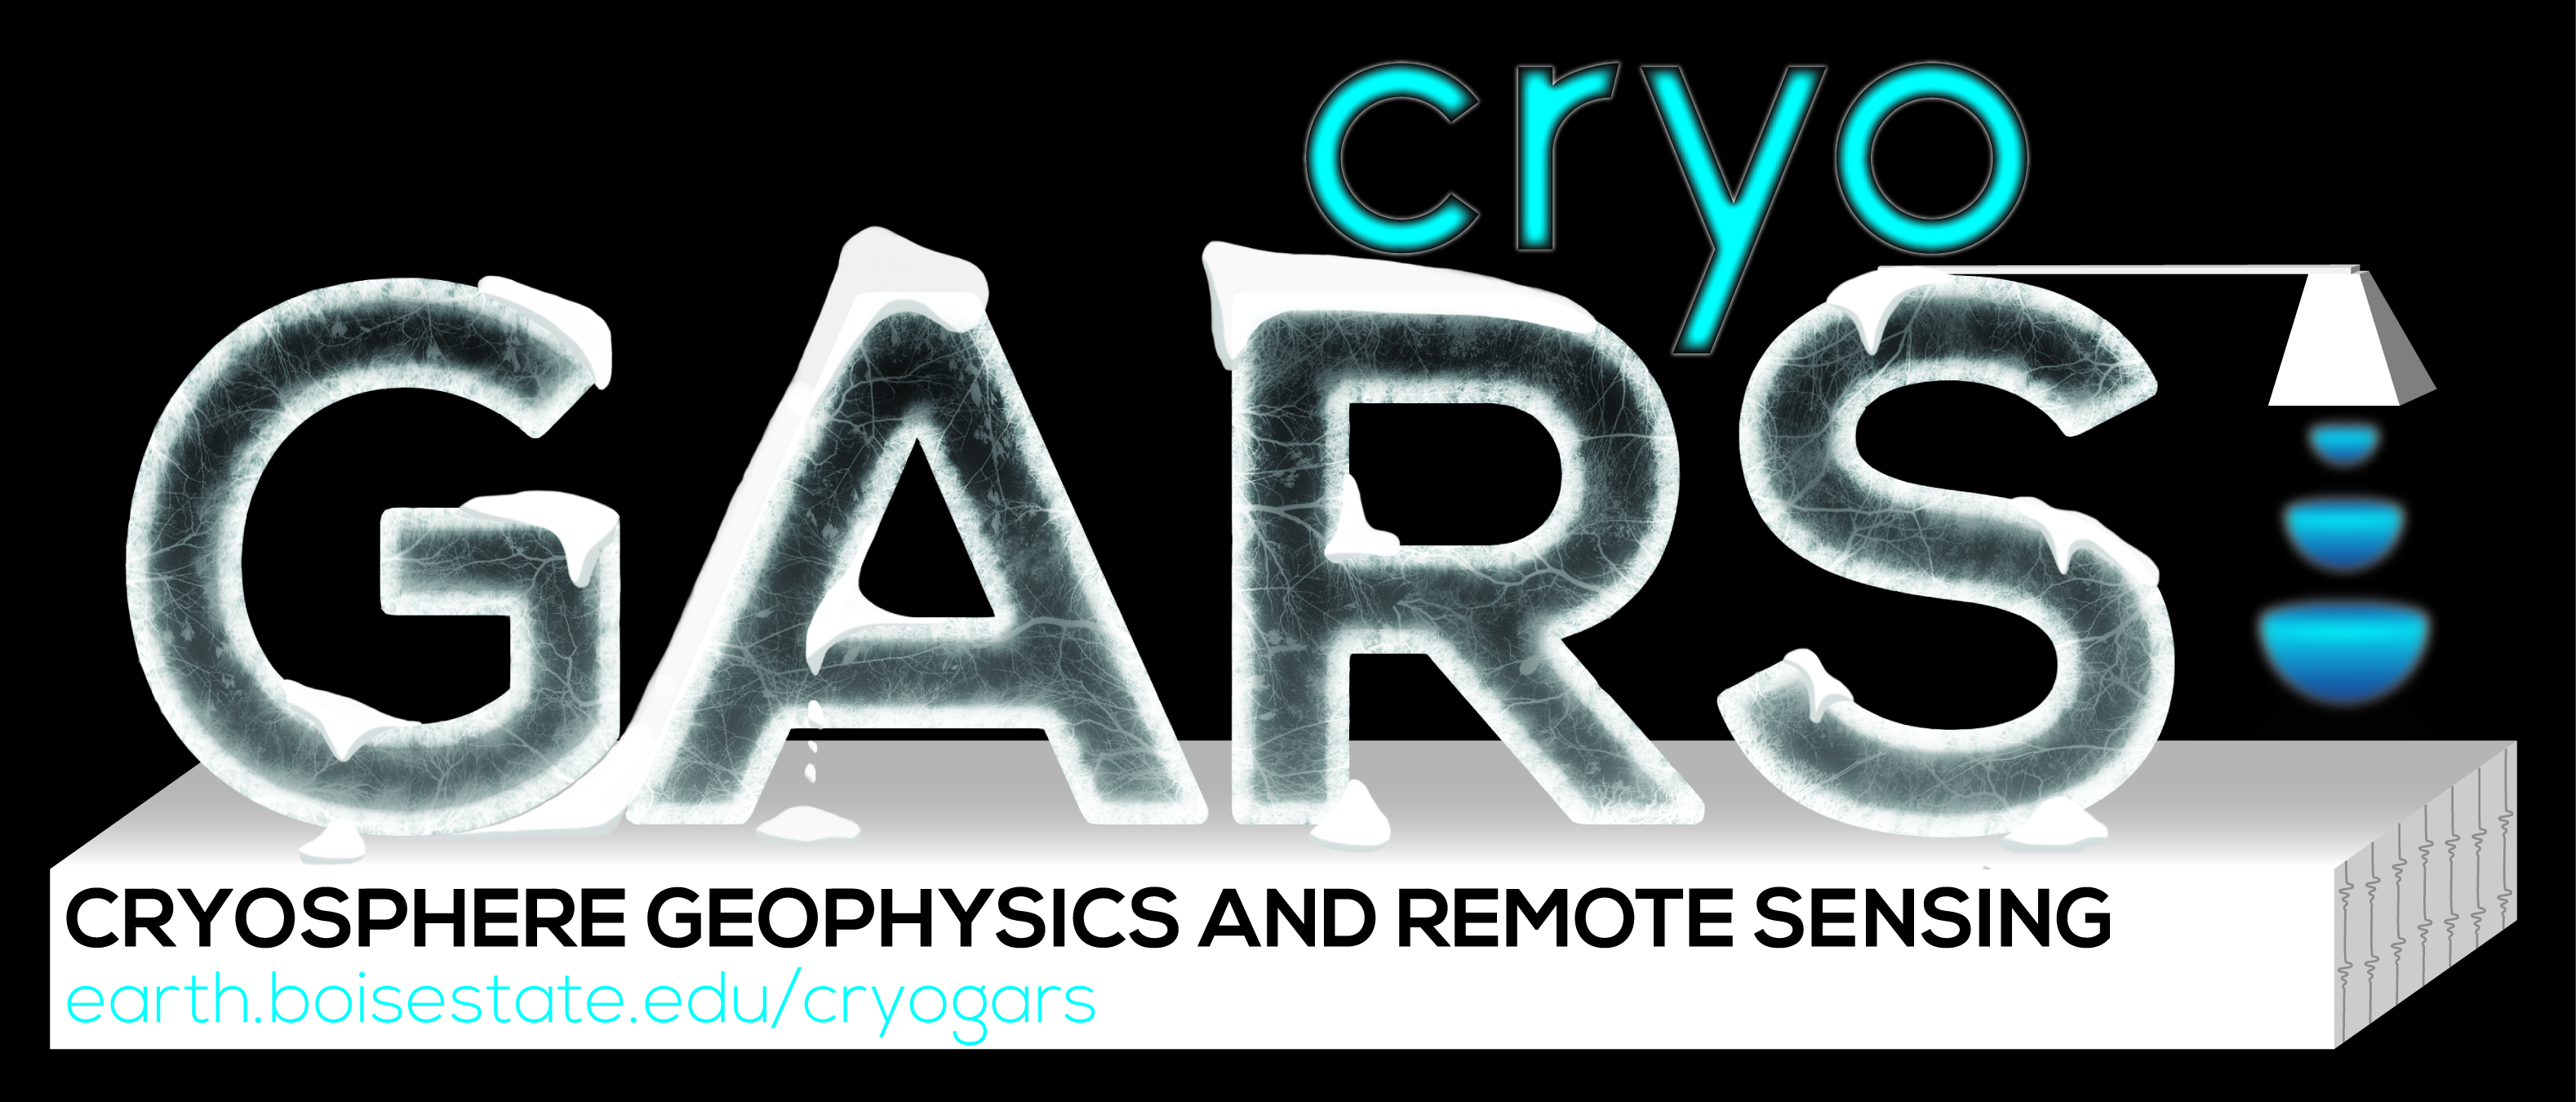
\includegraphics[width=6in]{CryoGARSLogo.jpg}

\section{Introduction}

I am submitting this retrospectus/prospectus during Fall 2018, to request feedback from the Tenure and Promotion Committee, and to signal my intent to apply for promotion to Professor in Fall 2019.  I began as an Assistant Professor at Boise State in August 2008, and received tenure and promotion to Associate Professor in July 2013.

This document outlines my long-term goals as a faculty in the Department of Geosciences at Boise State University, followed by a high-level summary of major accomplishments since tenure, and planned actions over the next five years, in the three areas of teaching, service, and research.  An appendix is included that lists some major external service, awards, a summary of research funding, and peer-reviewed publications since tenure.

\section{Goals}

The following three sections outline my goals for maintaining tripartite success as a faculty member of the Geosciences Department at Boise State.  These goals are long-term, and ones that I will continue to work towards throughout my career.

\subsection{Teaching}
My goals for teaching include continuing to improve the computational and quantitative skills of our undergraduate and graduate students, and continuing to improve each year myself as a teacher.  I want to develop and deliver courses that contribute to student learning across the department, and contribute to meeting the PLOs of all of our programs.  Field-based education is important to me, and I want to help deliver capstone field-based experiences, and contribute to and align with the department's new modular field camp approach.  

Active learning strategies and using metacognition approaches in the classroom are areas that I plan to continue to expand my use of.  I am a life-long student and will continue to seek opportunities to get additional training on effective teaching strategies.  Mentoring students is a high priority for me, including involving undergraduates in research, advising graduate students, and actively partipating on graduate student committees across the department.  Training the next generation of scientists, whether or not my students remain in the Cryosphere field, is one of my most important goals.

\subsection{Service}

My Service goals include contributing to the goals of the department, college, university, and the Cryosphere education and research community.  I want to help foster the cryosphere research and education community within Idaho, and take on leadership roles within the international snow community.  This requires finding a balance between efforts in all areas, and carefully choosing opportunities where I can most efficiently and effectively make an impact.

\subsection{Research}

In my specific area of research, I see the community approaching a required paradigm shift.  Previous approaches to forecasting water resources and natural hazards, related to snow and ice, have focused on historical records and index observations made at a handful of locations.  These approaches were necessary due to limited available information, limited understanding of the physical processes, and limited computational resources.  They also require the assumption of a stationary climate, and this poor assumption continues to have an ever increasing impact.  A paradigm shift, from index-based approaches, to spatiotemporally distributed monitoring approaches, is required; fortunately we are on the brink of such a leap, with available remote sensing and ground based information, along with computational resources, growing exponentially.  

The great increases in data and computing are allowing improvements in our understanding of the primary physical processes, and will lead to a shift to spatially distributed, high spatial and temporal resolution products of snow and ice properties to be used operationally in the future.  Fusion of information from 3 different areas is required to produce accurate estimates at the necessary spatiotemporal resolutions and extents: \textit{remote sensing}, \textit{modeling}, and 
\textit{ground-based observations}.  Strategies in these three areas have different advantages and disadvantages in terms of their cost, resolution, extent, and accuracy, and bridging the gap between scales will be an important component of the solution.

Much of my graduate research and pre-tenure focus was on the development of new tools for rapidly and accurately measuring snow properties from the ground.  I used these tools to study spatial variability of snow properties from the centimeter to 10 kilometer scale.  Since tenure, a major goal has been to push my work to larger, more societally relevant scales, which required more emphasis on larger field expeditions, airborne and satellite-based remote sensing, and developing partnerships with atmospheric and land surface modeling groups.  Near-realtime use of satellite remote sensing products, ground-based observations, in a modeling framework, to produce operational snow products, is a long-term goal.  This will require dedicated efforts in all three of these areas, and should involve interdisciplinary approaches that include collaborations with faculty across both the department and campus.

\section{Accomplishments}

This section highlights my major accomplishments that align with the above goals, in the three areas of Service, Teaching and Research, since I received tenure in 2013.  The end of the document lists a summary of research funding and selected recent external service, awards and publications.

\subsection{Service}

Service at the department, university, and international level is important to me.  At the departmental level, I have been a committee member of all four previous geophysics faculty searches, which now encompass our entire geophysics group within the department.  Our group has seen a great deal of turnover since I arrived in 2008, but I believe our current young group will be stable and will work well together; I am excited to continue to build our geophysics community within the department.  

I have been an active member of the Graduate Program Committee, serving from 2012-2015, and now filling in again during Jeff's sabbatical.  I am currently a member of the Geosciences Tenure and Promotion Committee, 
and was the department seminar coordinator for 2017-18.  At university level I have served on the COAS curriculum committee, and am currently a steering committee member for the new interdisciplinary \textit{Ph.D. in Computing} program.  I have served on the hiring committee for the COAS Instrumentation Shop, and I maintain a pool of survey-grade GPS instruments, and avalanche safety equipment.  This year I set up a UAV cost center, to facilitate the use of larger payload UAVs by faculty within the department and university.

I am an Ambassador for the Winter Wildlands Alliance, which is the parent organization for the nationwide SnowSchool program.  I develop curriculum and train volunteers for this program that reaches over 2,500 K-12 students each year in the Treasure Valley; the nationwide SnowSchool program has over 50 sites across the country.  I am a board member and instructor for the International Snow Working Group for Remote Sensing (ISWGR), for which I am on the executive committee and was recently voted incoming chair.  I am a board member of the American Institute for Avalanche Research and Education (AIARE), and give annual talks at the Sawtooth Avalanche Center professional development seminars.  I chair sessions at the American Geophysical Union (AGU) Fall meeting and International Snow Science Workshop (ISSW), and am an active reviewer for over 10 high quality journals.  I recently became an editor for \textit{Nature Scientific Reports}, and was on the review panel for the NASA Earth Venture Mission, a competition for satellite mission concepts.

\subsection{Teaching}

My teaching has been primarily focused at the graduate level.  \textit{GEOPH 422/522: Data Analysis and Geostatistics} is a course that I developed, after discussing departmental needs with faculty.  This fall I am teaching it for the 9$^{th}$ time, and it has become a requirement for the M.S. Hydrology degree.  The new efforts by Dylan and Karen to improve computational literacy in the department will make this course an opportunity for more of our advanced undergraduates.  Currently the enrollment is 10-15 graduate students every fall, with 1-2 occasional advanced undergraduates.  Based on feedback, I have broadened the exposure to different programming languages, by including a module covering \textit{R}, as this language is widely used especially in Geology.  

With over 1/3 of our graduate students currently doing research connected to snow, my spring course \textit{GEOPH 466/566: Snow and Ice Physics} has had enough enrollment to offer every other year, with 5-15 students enrolled, typically a mix of undergraduates and graduate students (7 graduate, 6 undergraduate in 2016).  This course includes both classroom and field-based components, and covers many of the PLOs that our field camps and geophysics courses target.  Interestingly, the undergraduates in this course have almost all come from outside the department, likely due to limited flexibility / electives in our undergraduate curriculum.  

I am currently working on aligning this course's field component with the goals and PLOs of the new departmental initiative for a modular field camp.  I am hoping that this will provide an opportunity to engage more of our undergraduate population, if this course could fill part of a field camp requirement; I think this course can meet the same PLOs of field camp in a setting where students can directly observe many processes common to geosciences, since the spatial and temporal scales in snow are so much smaller.  A group of faculty have made great progress towards an interdisciplinary field camp model that would allow a common set of PLOs to be achieved through a broad set of field modules.

During odd years in the spring, I have taught the core Geophysics course, \textit{GEOPH 502: Properties and Processes of the Earth II}, a field methods course, \textit{GEOPH 567: Snow Science Field Methods}, and have participated in the Faculty Incentive Program through teaching buy-out.  My teaching buy out in Spring 2017 allowed me to co-lead a 3000 km snowmobile traverse across the Greenland Ice Sheet, and to co-lead the month-long 2017 NASA SnowEx remote sensing campaign.  

A large component of my teaching workload is mentoring students.  I currently am primary advisor for 5 Ph.D. students, 1 MS student, and 1 undergraduate; since tenure I have maintained 5-12 students within my group.  I meet for one hour weekly 1-on-1 with each student, and hold weekly group meetings.  I am currently actively serving on more than 10 graduate student committees. 

I consider myself a lifelong student, and actively seek opportunities to improve my teaching.  I have integrated active learning strategies in both of my primary lecture courses; each course is approximately 50\% hands-on.  In the past year, I have attended teaching trainings and discussions through the \textit{Software Carpentry} program, and participated in the two-day National Association of Geoscience Teachers (NAGT) workshop this fall.  I attended a week long programming workshop at University of Washington, \textit{Geohackweek}, and a one week InSAR workshop at UNAVCO, as well as a CTL course for adapting courses for students with disabilities.

\subsection{Research}

My research program includes projects that focus on measuring snow properties and understanding snow physical processes, spanning a wide range of scales.  My research team, the Cryosphere Geophysics And Remote Sensing (CryoGARS) group, uses geophysics and remote sensing to tackle science questions about the \textit{Cryosphere}, or the areas of our earth where water exists in a frozen state.  My research is funded by NASA, NSF, DoD, Transportation Departments in several different states, and industry partners, and I currently have 10 active research grants, being carried out by myself, 7 graduate students and 1 undergraduate.  

In 2017 I co-led a large NASA snow remote sensing field experiment, with colleagues from the U.S. Army Cold Regions Research and Engineering Lab (CRREL), USFS, and NASA Goddard.  We received a NASA award for a successful month-long campaign, which involved over 100 scientists worldwide and 5 different NASA aircraft, with 10 airborne instruments.  This coming winter I have been named Project Scientist for the 2019 NASA SnowEx effort.  The goal of the 5-year NASA SnowEx effort is to collect the data necessary for a compelling satellite mission concept proposal, for monitoring snow globally from space.

In order to achieve distributed estimates of snow properties, at the global scale at the required spatial and temporal resolutions, advances in snow remote sensing, ground-based observations, and modeling are required.  Since receiving tenure, I have put significant effort into both maintaining effort in fundamental understanding of snow physics at the hillslope and watershed-scale, while expanding the scale of investigation to more societally-relevant extents, through improvement of remote sensing and modeling.  Published journal articles by our research group are summarized below.

Microscale snow properties have a large influence on snow remote sensing and liquid water movement, and we continue to improve our ability to rapidly measure snow microstructure and layering \citep{Havens:2013,Hagenmuller:2018}.  We have improved our understanding of the role of liquid water movement within snow at the centimeter - hillslope scale \citep{Eiriksson:2013,Heilig:2015}, including a paper in GRL with faculty authors from all 3 areas of Geosciences \citep{Evans:2016}.  We have made progress on improving the accuracy of snow and ice properties, and developed oil spill detection capability, from ground-based radar 
\citep{Bradford:2016,Rutter:2016,Pegau:2017}, and developed a new radar system for calibration of airborne and satellite-based 
snow radar \citep{Kim:2018}.

Distributed energy balance modeling at the hillslope scale led to improved understanding of the role of solar radiation and ground-water recharge in shallow snow at the rain-snow transition \citep{Kormos:2014b,Kormos:2014,Kormos:2015}.  New tools for rapidly measuring snow depth in the field enabled the study of the temporal evolution of snow patterns at the watershed scale \citep{Anderson:2014}, and the value of long term watershed scale monitoring was documented \citep{McNamara:2017}.  We have made progress in developing approaches for avalanche detection using infrasound \citep{Havens:2014}.

Airborne LiDAR has proven itself as a valuable tool for mapping snow depth distributions, leading to improved understanding of LiDAR errors and meter-to kilometer-scale snow patterns \citep{Tinkham:2013,McCreight:2014,Tinkham:2014}.
At larger scales, we have improved downscaling approaches that merge multiple satellite snow remote sensing products \\
\citep{Walters:2014}, and compared snow products from modeling, LiDAR, and field observations to improve uncertainty estimates 
and understanding of snow distribution at the regional scale \citep{Hedrick:2015}.  More recently, we are using snow depth estimates from airborne LiDAR to improve high-resolution physics-based snow modeling at the watershed scale \citep{Hedrick:2018}.

Finally, a collaborative NSF Arctic Natural Sciences grant, between Boise State, Dartmouth College, and University of Maine, provided funding over 3 years to perform a 3000+ km traverse across the Western Greenland Ice Sheet.  We recovered 15 shallow cores for geochemistry analysis \citep{Graeter:2018} and performed ground based radar surveys between coring sites.  This project is producing snow accumulation rate estimates and past melt records for an important area of the ice sheet that previously was poorly understood. Through comparison to airborne radar and climate models \citep{Lewis:2017} we are improving understanding of the surface mass balance that is controlling the contribution of the ice sheet to sea level rise.  Future work will include application of our ice core laser tomography system \citep{Mikesell:2017} to surface mass balance studies using ice and firn cores.

Other publications of note since tenure include two book chapters \citep{Marshall:2015,Arenson:2015}, two technical reports \citep{Havens:2014b,Rott:2013}, and two published/archived datasets \citep{Elder:2018,Brucker:2018}.  

\section{Planned Actions}

Over the next 5 years, I plan to continue to improve in all three areas of teaching, service and research.  I plan to complete my Software Carpentry instructor training, and contribute to future BSU-led Software Carpentry Workshops.  I will continue to improve my teaching, through application of effective teaching practices. I learned many new techniques during the recent NAGT workshop, as well as during the Software Carpentry trainings and the UW Geohackweek.  I plan to align my snow field course with the departmental PLOs for the modular field camp experience.  I would like to have more undergraduates from the department in my courses, which I think can be achieved through the increased computational literacy within the department, preparing more undergraduates for \textit{Data Analysis and Geostatistics}, and through alignment of \textit{GEOS 366 / GEOPH 566: Snow Physics and Avalanche Fundamentals} with the modular field camp requirement.  I also plan to deliver a hands-on graduate-level snow modeling course in Fall 2019, and develop a graduate level InSAR course for Fall 2020.

In the area of service, I plan to lead the 2019 NASA SnowEx campaign, and I hope to take a leadership role in a future snow satellite mission proposal in the next 5 years.  I plan to continue to grow our network of snow monitoring sites, and I plan to prepare to take advantage of upcoming snow-related satellite missions, such as IceSat2 and NISAR.  I want to continue to foster a geophysics community within the department, and in particular, help mentor our two new young geophysicists that will join our group in January.  

A strong snow modeling group has recently been developed at the USDA Northwest Watershed Research Center, headed by Danny Marks, and includes 4 of my recent graduate students.  One of my primary efforts in the near future is to integrate the advances in snow remote sensing that are occurring through the NASA SnowEx mission, with the cutting-edge high-resolution modeling work this group is doing.  In particular, I hope to build the infrastructure to take advantage of the NISAR satellite, launching in 2021, that will provide the L-band InSAR data needed to map snow water equivalent from space.  Large HPC resources will be required, including resources for cloud-based computing, as NISAR will produce 100 Tb of data per day.

\pagebreak

The primary risk for my success is that my research group could grow too quickly and exceed the size that is manageable, with the current level of university support.  This problem occurred previously to me, about 5 years ago, and I consciously reduced my group size at that time, when it was clear that university support was not available to support a larger group.  I realize that my number of active projects (10) has again approached a high level, and therefore I will focus on these funded projects, rather than additional proposals, at this time.

I look forward to feedback from the Tenure and Promotion Committee, the Chair, and the College. 

\vspace{0.5cm}

Sincerely,


\includegraphics{sig.png}
















\vspace{0.25in}

\begin{minipage}{0.70\linewidth}
Associate Professor \\
  \href{http://earth.boisestate.edu/cryogars/}{Cryosphere Geophysics And Remote Sensing (CryoGARS) group} \\
  Department of Geosciences and CGISS, Boise State University \\
  Environmental Research Building (ERB) 1104 (lab), 3155 (office) \\
  1910 University Drive \\
  Boise, ID  83725
\end{minipage}
\begin{minipage}{0.30\linewidth}
  \begin{tabular}{l}
     (208) 426-1416 (office) \\
     (303) 859-3106 (cell) \\
    \href{mailto:hpmarshall@boisestate.edu}{hpmarshall@boisestate.edu} \\
    \href{http://cgiss.boisestate.edu/~hpm}{cgiss.boisestate.edu/$\sim$hpm} \\
  \end{tabular}
\end{minipage}

\pagebreak

\section*{Research Funding Summary / Selected External Service / Awards}
\begingroup
\renewcommand\arraystretch{1}
\begin{longtable}{p{0.7in}|p{5.7in}}
2005-2018 & Awarded/managed over \$8 million in research funding from NASA, NSF, DoD, DOTs \\ 
2018-2019 & Project Scientist for 2019 NASA SnowEx mission \\
2018 & NASA Robert H. Goddard Team Award: SnowEx Year 1 Organizing Team \\
2018 & Joel Gongora, Ph.D. student, NASA Earth \& Space Sciences Fellowship (51 nationwide) \\
2018 & Tate Meehan, Ph.D. student, Idaho Space Grant Consortium Fellowship \\
2017 & Joel Gongora, Ph.D. student, Idaho Space Grant Consortium Fellowship \\
2017 & Co-lead for 2017 NASA SnowEx, largest seasonal snow remote sensing effort in 15 years \\
2016 & NASA Earth Venture Mission Panel Member (satellite proposals) \\
2015- & Education board member and Incoming Chair, NASA international Snow Working Group for Remote Sensing (iSWGR) \\
2012 & Timeless Award, University of Washington, 1 of 150 College of Arts and Sciences alumni  \\
& awarded from UW history on 150th yr anniv. (1861-2011), 1 of 3 from Physics \\
2012 & Andrew Hedrick, M.S. student, \textit{American Avalanche Assoc. Graduate Student Grant} \\
2012 & Scott Havens, Ph.D. student, \textit{$1^{st}$ place poster NSF/NASA EPSCoR annual meeting} \\
2012 & Kris Burch, Lloyd Lowe II, Kolton Drake, Undergrads, \\ 
& \textit{Best Senior Project, BSU College of Engineering} \\
2008-2012 & Cryosphere Section Representative, Fall AGU meeting \\
2011 & NASA Senior Review Panel Member (all current Earth Science satellite missions)
\end{longtable}
\endgroup




\section*{Selected Refereed Publications Since Tenure \\ \small{[h-index=20, i10-index=32, citations=1145]} \\
\hspace{2cm} \textit{[Since tenure (2013): h-index=17, i10-index=25, citations=804]} }
\setlength{\extrarowheight}{10pt}

\begin{longtable}{p{0.4in}|p{6.2in}}
2018 & \bibentry{Hedrick:2018} \\
 & \bibentry{Graeter:2018} \\
 & \bibentry{Kim:2018} \\
& \bibentry{Hagenmuller:2018} \\
2017 & \bibentry{Mikesell:2017} \\
& \bibentry{Lewis:2017} \\
& \bibentry{McNamara:2017} \\
& \bibentry{Pegau:2017} \\
2016 & \bibentry{Evans:2016} \\
& \bibentry{Rutter:2016} \\
& \bibentry{Bradford:2016} \\
2015 & \bibentry{Heilig:2015} \\
& \bibentry{Kormos:2015} \\
& \bibentry{Hedrick:2015} \\
2014 & \bibentry{Kormos:2014} \\
& \bibentry{Walters:2014} \\
& \bibentry{Havens:2014} \\
& \bibentry{Anderson:2014} \\
& \bibentry{Tinkham:2014} \\
& \bibentry{McCreight:2014} \\
& \bibentry{Kormos:2014b} \\
2013 & \bibentry{Havens:2013} \\
& \bibentry{Eiriksson:2013} \\
& \bibentry{Tinkham:2013} \\
\end{longtable}

\section*{Refereed Book Chapters / Technical Reports}
\begin{longtable}{p{0.3in}|p{6.2in}}
2015 & \bibentry{Marshall:2015} \\
 & \bibentry{Arenson:2015} \\
2014 & \bibentry{Havens:2014b} \\
2013 & \bibentry{Rott:2013} \\
\end{longtable}

\pagebreak

\section*{Archived Datasets}
\begin{longtable}{p{0.3in}|p{6.2in}}
2018 & \bibentry{Elder:2018} \\
2018 & \bibentry{Brucker:2018} \\
\end{longtable}


\nobibliography{mypubs}
\end{document}


